\begin{figure}
\centering
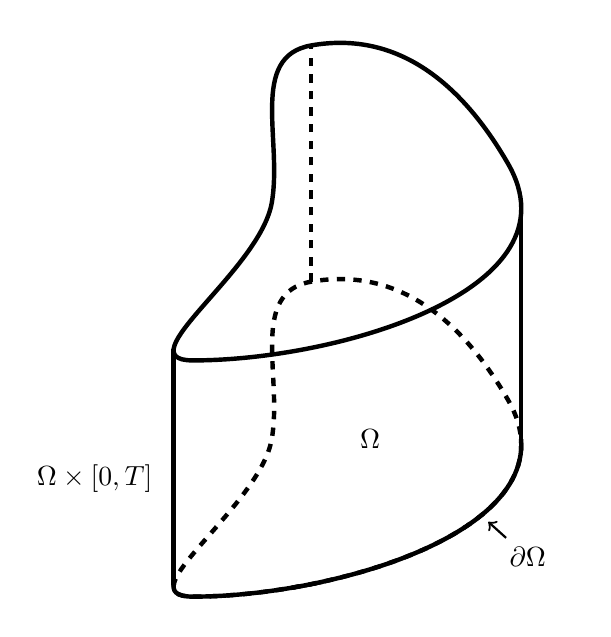
\begin{tikzpicture}[scale=0.5]
% TEXT
\node at (-0.5,3) (domain_time) {$\Omega \times [0,T]$};
\node at (6.5,4) (domain_top) {$\Omega$};
\node at (10.5,1) (domain_boundary) {$\partial \Omega$};
\draw [thick, ->] (domain_boundary) -- (9.5,1.9);
\begin{scope} % Top domain
\draw[ultra thick]
(2,6) 
to [out=0,in=300] (10,11)
to [out=120,in=10] (5,14)
to [out=190,in=80] (4,10)
to [out=260,in=180] (2,6);
\end{scope}
\begin{scope} % Bottom domain - solid
\clip (4.5,0) rectangle (10.4,4);
\draw[ultra thick]
(2,0) 
to [out=0,in=300] (10,5)
to [out=120,in=10] (5,8)
to [out=190,in=80] (4,4)
to [out=260,in=180] (2,0);
\end{scope}
\begin{scope} % Bottom domain - solid
\clip (0,0.3) rectangle (6,-0.3);
\draw[ultra thick]
(2,0) 
to [out=0,in=300] (10,5)
to [out=120,in=10] (5,8)
to [out=190,in=80] (4,4)
to [out=260,in=180] (2,0);
\end{scope}
\begin{scope} % Bottom domain - dashed
\draw[ultra thick, dashed]
(2,0) 
to [out=0,in=300] (10,5)
to [out=120,in=10] (5,8)
to [out=190,in=80] (4,4)
to [out=260,in=180] (2,0);
\end{scope}
\draw[ultra thick] % Left straight line
(1.5,0.3)
to [out=90,in=270] (1.5,6.3);
\draw[ultra thick] % Right straight line
(10.33,4)
to [out=90,in=270] (10.33,10);
\draw[ultra thick, dashed] % Top straight line
(5,8)
to [out=90,in=270] (5,14);
\end{tikzpicture}
\caption{The spatial and temporal domain $\Omega^+ = \Omega \times [0,T]$ for the partial differential equations in the black oil model, Equation (\ref{eq:black_oil_model}). The spatial domain has border $\partial \Omega$.} \label{fig:spatial_temporal_domain}
\end{figure}